\documentclass{article}
\usepackage[utf8]{inputenc}
\usepackage{hyperref}
\usepackage{csquotes}
\usepackage{graphicx}

\graphicspath{ {res/} }
\hypersetup{
    colorlinks=true,
    linkcolor=none,
    urlcolor=magenta,
}

\renewcommand{\familydefault}{\sfdefault}
\newcommand{\chikalegal}{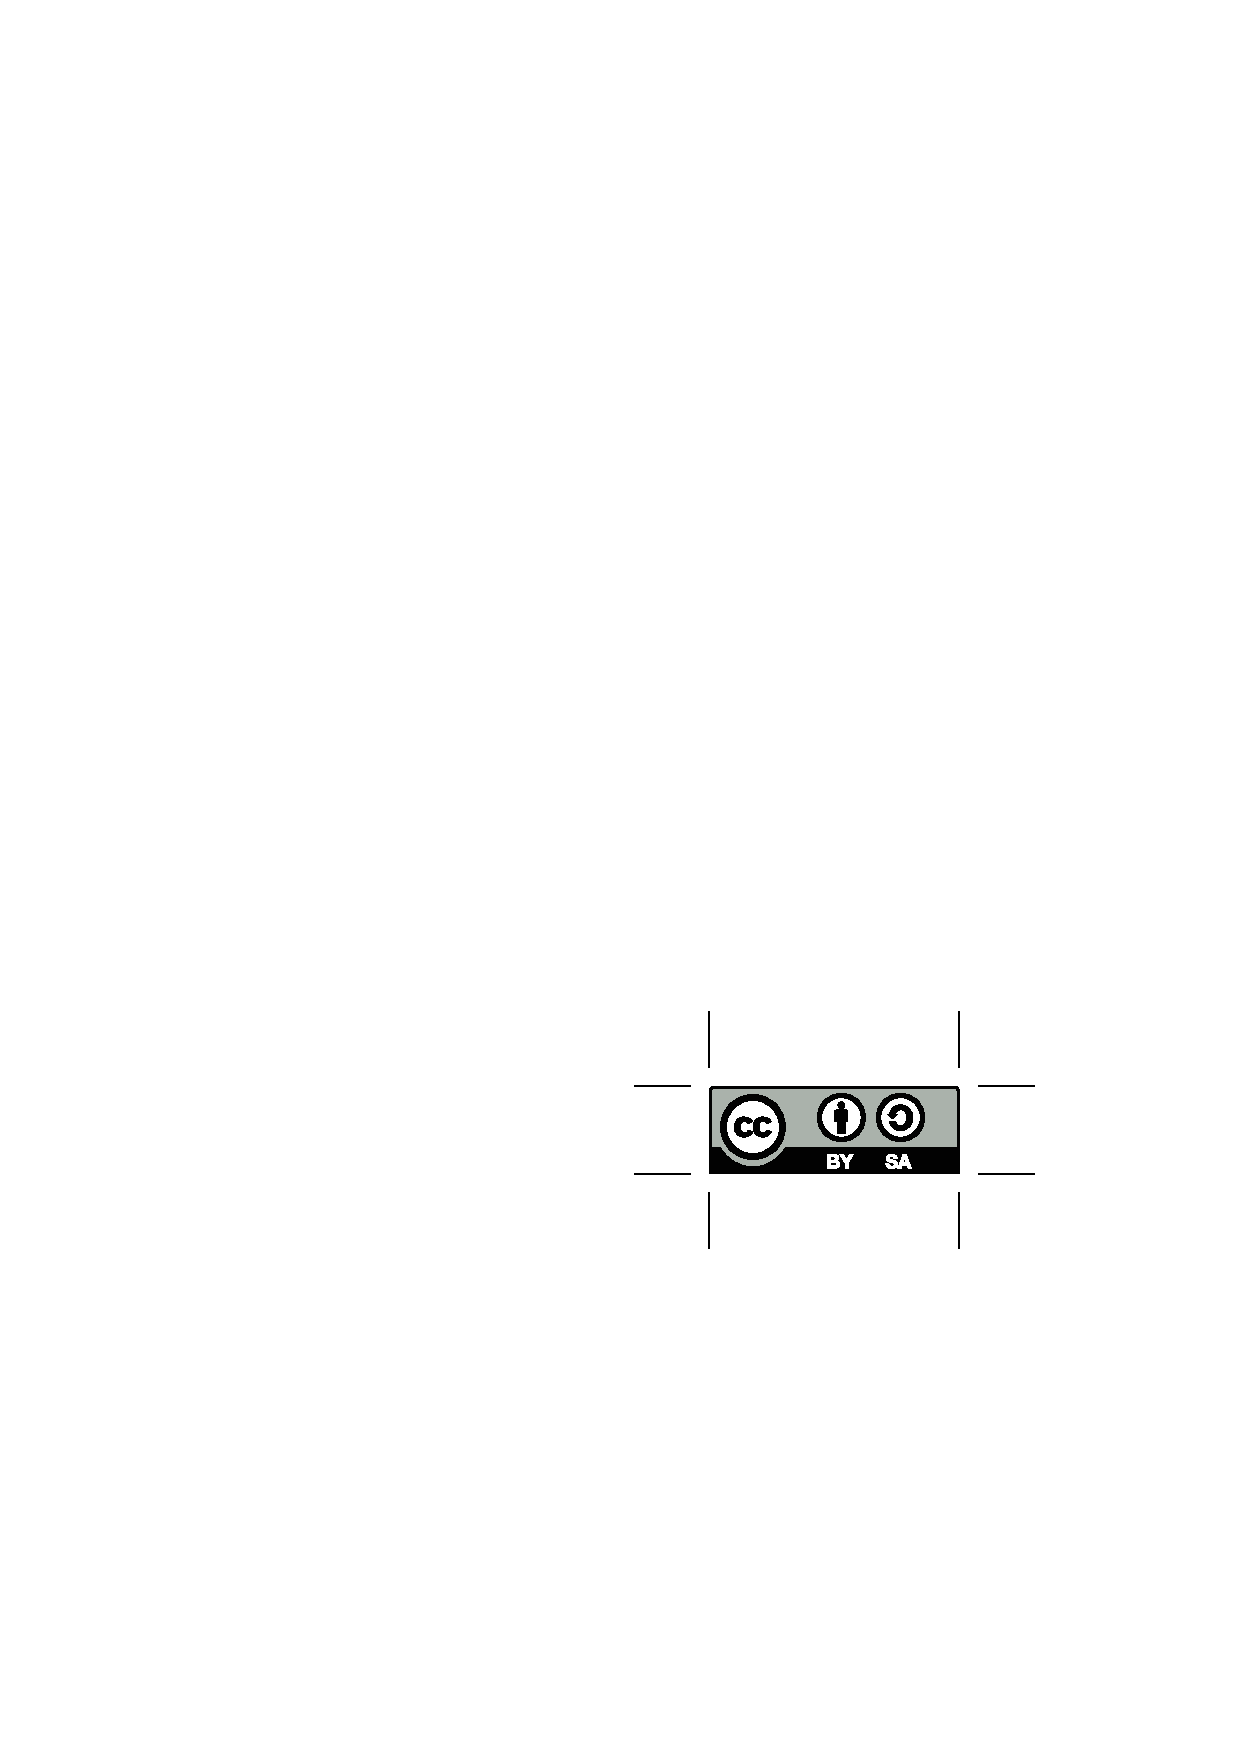
\includegraphics[scale=0.75]{by-sa}

This work is licensed under the Creative Commons Attribution-ShareAlike 4.0 International License. To view a copy of this license, visit \url{http://creativecommons.org/licenses/by-sa/4.0/} or send a letter to Creative Commons, PO Box 1866, Mountain View, CA 94042, USA. Copyright \copyright~2019-\the\year~Chika Games.

The RPG Maker trademark and copyright are property of Enterbrain, Inc. and Kadokawa Corporation. All rights belong to their respective owners.}
\newcommand{\specpreamble}{\maketitle
\tableofcontents
\newpage
\chikalegal
\newpage}


\title{LCF Map Tree Specification (LMT)}
\author{Chika Games}

\begin{document}
\specpreamble

\section{Introduction}
LCF Map Tree files are used to store map properties, game start information, and map orderings for RPG Maker 2000/2003 games.

This specification is part of a larger collection that can be found at the following URL: \url{https://github.com/chika-games/RPG-Maker-Specifications}.

\section{Data Types}
This section describes the various data types that will be used throughout this specification.

Little-endian byte order is assumed for all types; the least significant byte is stored first, and the most significant byte is stored last.

Types may be appended with \textit{[n]} in order to denote a contiguous array of the type in question, where \textit{n} is the number of elements. For example, \textit{U8[4]} denotes an array of four unsigned 8-bit integers.

\subsection{Basic Data Types}
These types are considered \textit{primitive} as all other data types are constructed using these:

\begin{table}[h!]
\centering
\begin{tabular}{|l|l|}
\hline
\textbf{Type} & \textbf{Description}            \\ \hline
U8            & An unsigned 8-bit integer.      \\ \hline
U32           & An unsigned 32-bit integer.     \\ \hline
VINT          & An encoded integer (see below). \\ \hline
\end{tabular}
\end{table}

\subsubsection{Encoded Integers}
LCF files make extensive use of 7-bit encoded integers instead of more common fixed-length formats. These types of integers will only use the minimum number of bytes needed to encode a particular value. For example, 123456 will be encoded as two bytes. This helps reduce the overall size of LCF files.

Bytes will contribute up to seven bits worth of numerical information, and the eighth bit will indicate whether or not another byte is to follow.

Below is pseudocode for reading, decoding, and converting these encoded integers into a fixed-length (\textit{U32}) format:

\begin{lstlisting}[frame=single]
u32 read_variable_integer(reader) {
    u32 ret = 0;

    while true {
        u8 b = reader.read_u8();

        ret <<= 7;
        ret |= b & 0x7F;

        if (b & 0x80) == 0 {
            break;
        }
    }

    return ret;
}
\end{lstlisting}

\subsection{Compound Data Types}
These types are constructed using a combination of basic data types.

\subsubsection{STRING Type}
The \textit{STRING} type represents a length-prepended string of characters. These are used for all forms of textual data.

\textbf{Note:} Strings have no standard encoding. It is up to the runtime's discretion as to which encoding to use; this is typically based on the current operating system's locale. Japanese games will typically use \href{https://en.wikipedia.org/wiki/Shift_JIS}{Shift JIS}.

\begin{table}[h!]
\centering
\begin{tabular}{|l|l|l|}
\hline
\textbf{Field} & \textbf{Type}           & \textbf{Description}                             \\ \hline
Length         & \textit{VINT}           & The length of the string in bytes.               \\ \hline
Characters     & \textit{U8{[}Length{]}} & The array of characters that make up the string. \\ \hline
\end{tabular}
\end{table}

\section{LMT File Structure}
This section details the overall structure of an LMT file.

\begin{table}[h!]
\centering
\begin{tabular}{|l|l|l|}
\hline
\textbf{Field} & \textbf{Type}                       & \textbf{Description}                                       \\ \hline
Signature      & \textit{STRING}                     & The file's signature. Should always be "LcfMapTree".       \\ \hline
MapInfoCount   & \textit{VINT}                       & The number of info structures present.                     \\ \hline
MapInfos       & \textit{Map Info{[}MapInfoCount{]}} & An array of map information.                               \\ \hline
MapOrderCount  & \textit{VINT}                       & The number of map orderings present.                       \\ \hline
MapOrders      & \textit{VINT{[}MapOrderCount{]}}    & The hierarchical orderings of a game's maps.               \\ \hline
ActiveNode     & \textit{VINT}                       & For editor use only. The ID of the last active/edited map. \\ \hline
MapStart       & \textit{Map Start}                  & Game start information, such as starting positions.        \\ \hline
\end{tabular}
\end{table}

\section{Map Info Structure}
\section{Map Start Structure}

\subsection{Example Map Hierarchy}
Below is an example hierarchy to help illustrate various fields of an LMT file. Notice all maps are children to the root map.

\section{Tags}
\subsection{Map Info Tags}
\subsection{Map Start Tags}
\subsection{Music Tags}
\subsection{Encounter Tags}

\end{document}
